\documentclass[11pt]{article}
\usepackage[margin=1in]{geometry}
\usepackage[T1]{fontenc}
\usepackage{lmodern}
\usepackage{booktabs}
\usepackage{graphicx}
\usepackage{longtable}
\usepackage{array}
\usepackage{float}
\usepackage{caption}
\usepackage{xcolor}
\usepackage[hidelinks]{hyperref}
\captionsetup{font=small,labelfont=bf}
\setlength{\parindent}{0pt}\setlength{\parskip}{6pt}
\title{\textbf{Labor-Market Outcomes of Former Student-Visa Holders}\\[2pt]\large 2023 National Survey of College Graduates}
\author{Institute for Progress}
\date{September 14, 2026}
\begin{document}
\maketitle
\thispagestyle{empty}
\section*{Overview}
This report analyzes the labor-market outcomes of \textbf{student-visa entrants} --- people whose first U.S.\ visa was a student visa --- compared with \textbf{natives}, using the 2023 National Survey of College Graduates (NSCG) public-use microdata. The research and federal-support sections additionally distinguish those who are \emph{currently} on a student visa.\par
\section*{Data and definitions}
\begin{itemize}
\item \textbf{Source:} NCSES 2023 NSCG public-use file (Sept.\ 11, 2025 release); 94,606 respondents.
\item \textbf{Student visa entrants} = first U.S.\ visa was a student visa (\texttt{FNVSATP} code 3; n=8,577). \textbf{Native} = U.S.\ native, no entry visa (\texttt{FNVSATP} code L; n=69,286). Unless a section says otherwise, ``student visa'' columns refer to entrants, not to those currently on a student visa.
\item \textbf{Working universe} (all salary tables): full-time, full-year workers --- 50+ weeks/year (\texttt{WKSLYR}>49), 35+ hours/week (\texttt{HRSWK}>34), and non-missing salary (\texttt{SALARY}$\neq$9{,}999{,}998).
\item \textbf{Weights:} all population estimates use the survey weight \texttt{WTSURVY}; medians are weighted (\texttt{matrixStats::weightedMedian}).
\item \textbf{Self-employment rate} = self-employed workers (\texttt{EMTP} 12 or 13) as a share of \emph{all} workers in the group, i.e.\ self-employed $\div$ (self-employed $+$ not self-employed).
\item \textbf{Federal agency support:} whether the respondent's principal-job work was supported by a U.S. federal agency (\texttt{GOVSUP}) and, if so, which agencies (\texttt{FS*}, ``mark all that apply''). Agency shares overlap and need not sum to the ``any federal support'' figure.
\item \textbf{Basic / applied research:} whether the respondent spent at least 10\% of a typical work week on basic research (\texttt{WABRSH}) or applied research (\texttt{WAAPRSH}) on the principal job.
\item \textbf{Student-visa groupings} (research and federal-support sections): \emph{current student visa holders} = held a student/training visa on Feb.\ 1, 2023 (\texttt{VSATP}); \emph{student visa entrants} = first U.S.\ visa was a student visa (\texttt{FNVSATP}). Each is compared with all other full-time/full-year workers.
\item \textbf{Caveat:} the public-use file omits stratum/PSU identifiers, so these are point estimates without design-based standard errors; small cells (some industries and sender countries) are noisy.
\end{itemize}
\section{Headline salary comparison}
Among full-time, full-year workers, student-visa entrants have a substantially higher median salary than natives.
\begin{table}[H]
\centering
\caption{Median annual salary, full-time/full-year workers}

\begin{tabular}{lr}
\toprule
First visa type & Median salary\\
\midrule
Native & \$87,000\\
Student visa entrants & \$115,249\\
\bottomrule
\end{tabular}
\end{table}
\section{Salary by age (decade)}
\begin{table}[H]
\centering
\caption{Median salary by age bucket}

\begin{tabular}{lrr}
\toprule
Age bucket & Native & Student visa entrants\\
\midrule
20s & \$62,000 & \$81,896\\
30s & \$88,000 & \$117,522\\
40s & \$100,000 & \$130,000\\
50s & \$100,000 & \$124,729\\
60+ & \$99,945 & \$110,000\\
\bottomrule
\end{tabular}
\end{table}
\section{Salary by degree level}
\begin{table}[H]
\centering
\caption{Median salary by most-recent-degree type (BA / MA / PhD / Professional)}

\begin{tabular}{lrrrr}
\toprule
Visa type & BA & MA & PhD & Prof\\
\midrule
Native & \$80,000 & \$95,000 & \$112,000 & \$150,000\\
Student visa entrants & \$80,000 & \$125,000 & \$130,000 & \$112,321\\
\bottomrule
\end{tabular}
\end{table}
\section{Degree-level composition}
Student-visa entrants are far more concentrated in graduate degrees (MA/PhD) than natives.
\begin{table}[H]
\centering
\caption{Distribution of most-recent-degree type, by group (weighted shares within group)}

\begin{tabular}{lrr}
\toprule
Degree & Native share & Student-visa-entrant share\\
\midrule
BA & 65.1\% & 28.8\%\\
MA & 26.1\% & 47.2\%\\
PhD & 2.9\% & 19.0\%\\
Prof & 5.9\% & 5.0\%\\
\bottomrule
\end{tabular}
\end{table}
\section{Salary by industry}
\begin{table}[H]
\centering
\caption{Median salary by industry group (industries with very few international graduates --- Agriculture, Military, Wholesale Trade --- are excluded, per the source script)}

\begin{tabular}{lrr}
\toprule
Industry & Native & Student visa entrants\\
\midrule
Information & \$100,000 & \$186,434\\
Prof services & \$102,000 & \$140,000\\
Manufacturing & \$106,000 & \$130,000\\
FIRE & \$100,000 & \$120,551\\
Retail Trade & \$80,000 & \$110,000\\
Trans/WH, Util & \$101,000 & \$110,000\\
Public Admin & \$85,000 & \$99,288\\
Accom \& Food & \$63,820 & \$95,817\\
Other Services & \$58,000 & \$87,375\\
Ed and HC & \$72,500 & \$75,000\\
\bottomrule
\end{tabular}
\end{table}
\section{Salary by country of birth}
Top ten sending countries among student-visa entrants, ranked by estimated number of graduates.
\begin{table}[H]
\centering
\caption{Median salary and estimated graduate counts, top 10 countries of birth (student-visa entrants)}

\begin{tabular}{lrr}
\toprule
Country of birth & Median salary & Est. graduates\\
\midrule
India & \$146,000 & 372,042\\
China & \$125,000 & 303,420\\
Korea, South & \$75,686 & 64,307\\
Taiwan & \$106,390 & 55,029\\
Nigeria & \$80,000 & 48,554\\
Iran & \$110,000 & 46,698\\
Canada & \$120,000 & 46,615\\
Mexico & \$98,000 & 42,537\\
Japan & \$90,000 & 42,143\\
Germany & \$105,000 & 31,557\\
\bottomrule
\end{tabular}
\end{table}
\section{Research activity}
Student-visa entrants are more than twice as likely as natives to have research as a primary or secondary activity on their principal job.
\begin{table}[H]
\centering
\caption{Share whose principal-job primary or secondary activity is basic or applied research (ACTRES), weighted}

\begin{tabular}{lrrr}
\toprule
Visa type & Research (wt.) & No research (wt.) & Research rate\\
\midrule
Native & 4,356,564 & 31,448,588 & 12.2\%\\
Student visa entrants & 474,090 & 1,281,470 & 27.0\%\\
\bottomrule
\end{tabular}
\end{table}
\section{Basic and applied research}
Share of full-time/full-year workers who spend at least 10\% of a typical work week on basic or applied research, shown two ways: by whether the respondent is \emph{currently} on a student visa, and by whether their \emph{first} U.S.\ visa was a student visa. ``All other workers'' is everyone else (natives and other immigrants). The student-visa group leads on both measures under either definition.
\begin{figure}[H]
\centering
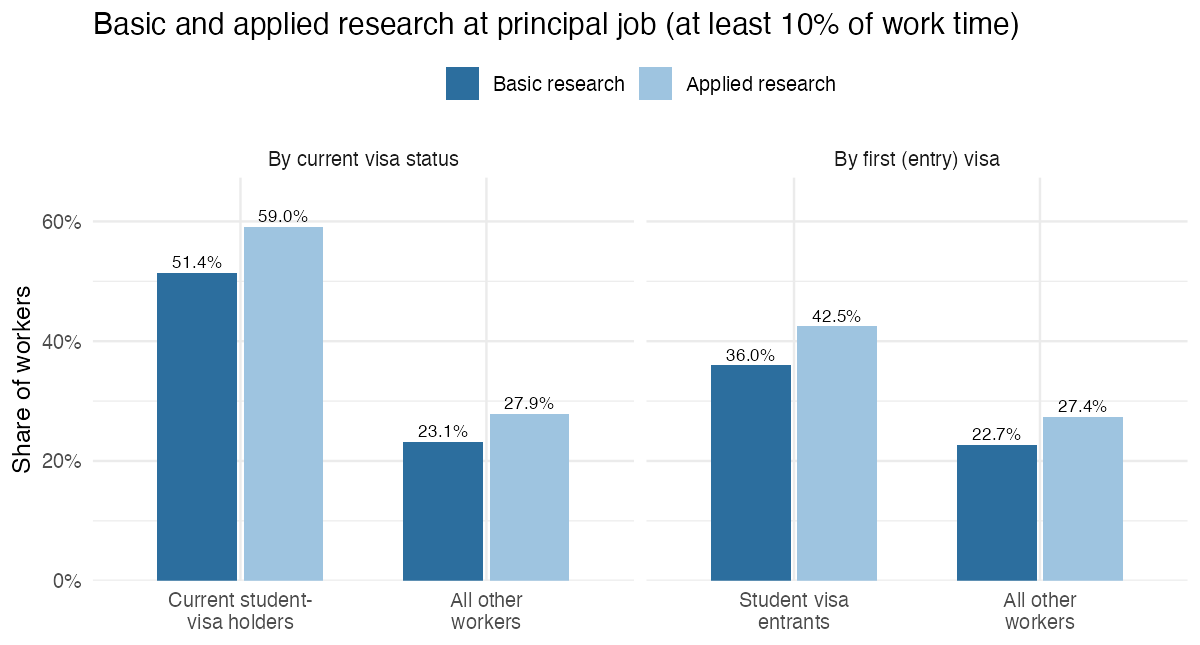
\includegraphics[width=0.98\textwidth]{figures/research_basic_applied.png}
\caption{Basic and applied research at the principal job (at least 10\% of work time)}
\end{figure}
\begin{table}[H]
\centering
\caption{Basic and applied research, by current student-visa status}

\begin{tabular}{lrr}
\toprule
Research activity & Current student visa holders & All other workers\\
\midrule
Basic research & 51.4\% & 23.1\%\\
Applied research & 59.0\% & 27.9\%\\
\bottomrule
\end{tabular}
\vspace{3pt}
{\footnotesize\itshape Universe: full-time/full-year workers. Unweighted n: current student visa = 557; all other workers = 64,072.}
\end{table}
\begin{table}[H]
\centering
\caption{Basic and applied research, by first-entry visa (whether the first U.S. visa was a student visa)}

\begin{tabular}{lrr}
\toprule
Research activity & Student visa entrants & All other workers\\
\midrule
Basic research & 36.0\% & 22.7\%\\
Applied research & 42.5\% & 27.4\%\\
\bottomrule
\end{tabular}
\vspace{3pt}
{\footnotesize\itshape Universe: full-time/full-year workers. Unweighted n: entered on student visa = 6,430; all other workers = 58,199.}
\end{table}
\section{Federal agency support}
Share of workers whose principal-job work is supported by each U.S.\ federal agency, shown two ways: by current student-visa status and by first-entry visa. Because work can be backed by more than one agency (``mark all that apply''), the agency rows overlap and need not sum to the ``any federal support'' row.
\begin{table}[H]
\centering
\caption{Federal agency support, by current student-visa status}

\begin{tabular}{lrr}
\toprule
Federal agency & Current student visa holders & All other workers\\
\midrule
Any federal support & 20.5\% & 11.2\%\\
NIH & 7.4\% & 1.0\%\\
NSF & 8.1\% & 0.4\%\\
Other agency & 2.4\% & 3.0\%\\
Defense (DOD) & 0.9\% & 2.6\%\\
HHS (excl. NIH) & 0.5\% & 1.8\%\\
Energy (DOE) & 1.9\% & 0.6\%\\
Education & 0.6\% & 1.8\%\\
NASA & 0.6\% & 0.4\%\\
\bottomrule
\end{tabular}
\vspace{3pt}
{\footnotesize\itshape Agencies overlap (mark all that apply). Unweighted n: current student visa = 618; all other workers = 68,052.}
\end{table}
\begin{table}[H]
\centering
\caption{Federal agency support, by first-entry visa}

\begin{tabular}{lrr}
\toprule
Federal agency & Student visa entrants & All other workers\\
\midrule
Any federal support & 10.9\% & 11.2\%\\
NIH & 3.6\% & 1.0\%\\
NSF & 2.0\% & 0.4\%\\
Other agency & 1.7\% & 3.0\%\\
Defense (DOD) & 1.2\% & 2.6\%\\
HHS (excl. NIH) & 1.1\% & 1.8\%\\
Energy (DOE) & 0.9\% & 0.5\%\\
Education & 0.8\% & 1.8\%\\
NASA & 0.5\% & 0.4\%\\
\bottomrule
\end{tabular}
\vspace{3pt}
{\footnotesize\itshape Agencies overlap (mark all that apply). Unweighted n: entered on student visa = 6,702; all other workers = 61,968.}
\end{table}
\section{Self-employment}
\begin{figure}[H]
\centering
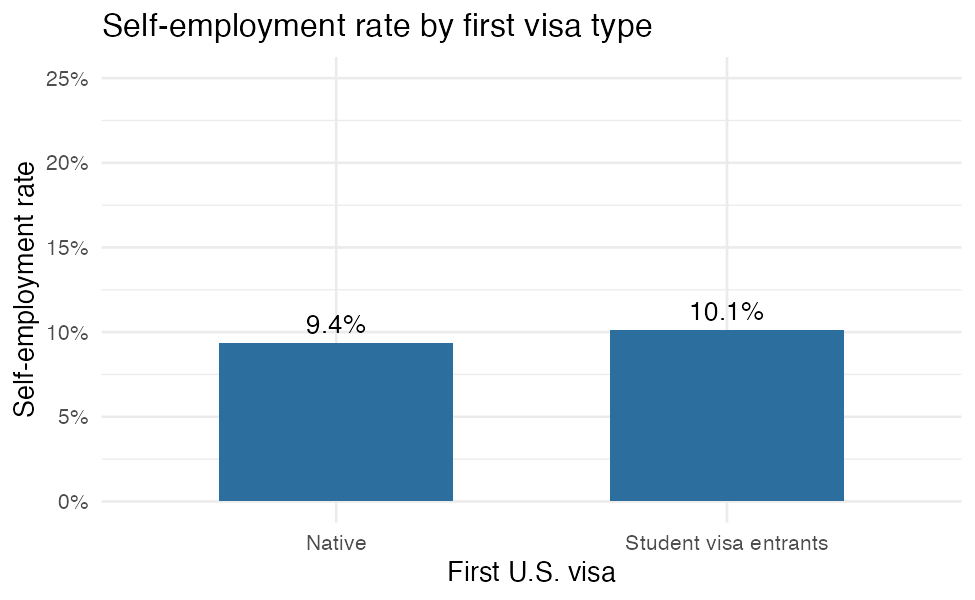
\includegraphics[width=0.8\textwidth]{figures/ent_by_first_visa.png}
\caption{Self-employment rate by first visa type}
\end{figure}
\begin{table}[H]
\centering
\caption{Self-employment rate by first visa type}

\begin{tabular}{lrrr}
\toprule
Visa type & Self-employed (wt.) & Not (wt.) & Rate\\
\midrule
Native & 4,606,497 & 44,579,039 & 9.4\%\\
Student visa entrants & 211,574 & 1,875,050 & 10.1\%\\
\bottomrule
\end{tabular}
\end{table}
\begin{figure}[H]
\centering
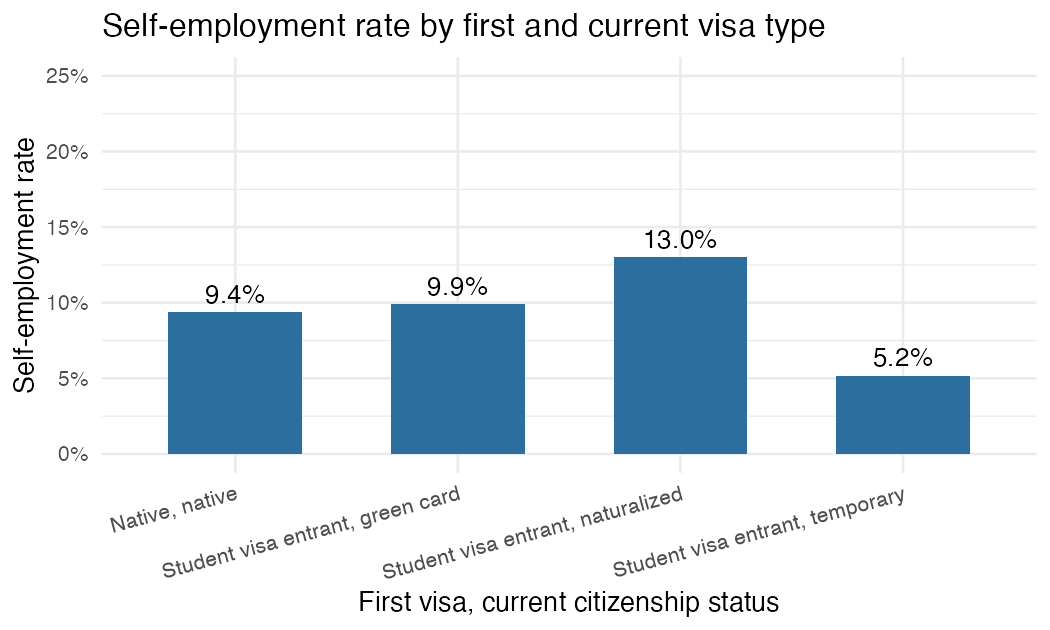
\includegraphics[width=0.8\textwidth]{figures/ent_by_first_current.png}
\caption{Self-employment rate by first and current visa/citizenship status}
\end{figure}
\begin{table}[H]
\centering
\caption{Self-employment rate by first and current status}

\begin{tabular}{lrrr}
\toprule
First visa, current status & Self-employed (wt.) & Not (wt.) & Rate\\
\midrule
Native, native & 4,599,686 & 44,555,832 & 9.4\%\\
Student visa entrant, green card & 54,170 & 493,032 & 9.9\%\\
Student visa entrant, naturalized & 129,346 & 864,618 & 13.0\%\\
Student visa entrant, temporary & 28,057 & 515,771 & 5.2\%\\
\bottomrule
\end{tabular}
\end{table}
\section{Current status of student-visa entrants}
Where student-visa entrants (full-time/full-year) stand today, by current citizenship status.
\begin{table}[H]
\centering
\caption{Current citizenship status of student-visa entrants (weighted)}

\begin{tabular}{lr}
\toprule
Current citizenship status & Weighted total\\
\midrule
naturalized & 993,964\\
green card & 547,203\\
temporary & 543,828\\
native & 1,629\\
\bottomrule
\end{tabular}
\end{table}
\appendix
\section{Unweighted sample sizes by industry}
Raw (unweighted) record counts underlying the industry salary table, showing why several industries are dropped.
\begin{table}[H]
\centering
\caption{Unweighted respondent counts by industry and group}

\begin{tabular}{lrr}
\toprule
Industry & Native & Student visa entrants\\
\midrule
Prof services & 11,258 & 2,103\\
Ed and HC & 11,658 & 1,524\\
Manufacturing & 7,209 & 1,151\\
FIRE & 3,150 & 470\\
Information & 1,248 & 295\\
Retail Trade & 1,251 & 216\\
Public Admin & 5,201 & 209\\
Trans/WH, Util & 1,535 & 126\\
Agriculture & 577 & 57\\
Accom \& Food & 689 & 54\\
Other Services & 962 & 54\\
Wholesale Trade & 496 & 50\\
Military & 153 & 1\\
\bottomrule
\end{tabular}
\end{table}

\end{document}

